\section{Approach}
\label{sec:approach}

Our approach accepts a set of projects as data sources and mines
API mapping between two different languages $L_1$ and $L_2$. 
As mined API mapping describes mapping relations of APIs between 
the two languages, this mapping is useful for language migration between the two languages. 
For each project used as a data source, our approach requires 
atleast two versions of the project (one version in $L_1$ and
the other version in $L_2$). Figure~\ref{fig:approach} shows
the overview of our approach.

First, our approach aligns client code in languages $L_1$ and $L_2$ 
so that the aligned source files implement similar functionalities 
(Section~\ref{sec:approach:acc}). Second, our approach mines 
mapping relations of API classes (Section~\ref{sec:approach:mappingtypes}). 
Finally, our approach mines mapping relations of API 
methods (Section~\ref{sec:approach:mappingtypes}) defined by the mapped
API classes.

\begin{figure}[t]
\centering
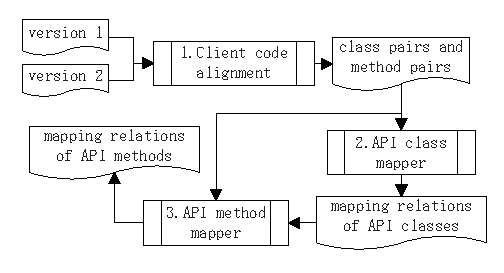
\includegraphics[scale=1,clip]{figure/approach.eps}\vspace*{-3ex}
 \caption{Overview of our approach}\vspace*{-3.5ex}
 \label{fig:approach}
\end{figure}

%-------------------------------------------------------------------
\subsection{Aligning Client Code}
\label{sec:approach:acc}

Initially, our approach accepts two versions of a project (one version in 
$L_1$ and the other version in $L_2$) and aligns classes and methods
of the two versions. Aligned classes or methods 
between the two versions implement a similar functionality. As they
implement a similar functionality, APIs used by these classes or methods can be
replaceable.

To align classes and methods of the two versions, our approach uses
name similarities between entities (such as class names or method names)
defined by the two versions of the project. In our approach, we have two
different kinds of entity names: entity names defined by the two versions
of the project and entity names of third-party libraries used by the two versions of the project.
The first kind often comes from the same programmer or the same team, or
programmers may refer to existing versions for naming entities such
as classes, methods, and variables. Therefore, name similarity is often 
reliable to distinguish functionalities of the first kind compared to the second
kind. Our approach uses Simmetrics\footnote{\url{http://sourceforge.net/projects/simmetrics/}}
to calculate name similarities.

Algorithm~\ref{alg:alignclasses} shows how our approach aligns
client code classes. The first step is to find
candidate class pairs by names. For two sets of classes ($C$ and
$C'$), the algorithm returns candidate class pairs ($M$) with
a similarity greater than a given threshold, referred to as \emph{SIM\_THRESHOLD}. 
As some projects may have many classes with the
same name, $M$ may contain more than one matching pair for a class in a version. 
To align those classes, our algorithm uses package names of
these classes to refine $M$ and returns only one matching pair with the
maximum similarity\footnote{For C\#, we refer to namespace names for
package names.}.

In each aligned class pair, our approach further aligns methods
within the class pair. The algorithm for methods is similar to the
algorithm for classes but relies on other criteria such as the number of parameters
and names of parameters to refine candidate method pairs. These candidates
may contain more than one method pair due to overloading.
For the example shown in Section~\ref{sec:example}, our approach
correctly aligns the class \CodeIn{IndexFiles} and the method
\CodeIn{main} in Java to the class \CodeIn{IndexFiles}
and the method \CodeIn{Main} in C\# as their names are quite
similar.
%-----------------------------------------------------------------
\subsection{Mapping API classes}
\label{sec:approach:mappingtypes} 

In this step, our approach mines mapping relations of 
API classes. As defined in Section~\ref{sec:mapping}, mapping relations of API classes are used
to translate variables. Consequently, our approach mines mapping
relations of API classes based on how aligned client code declares
variables such as fields of aligned classes, parameters of aligned methods
and local variables of aligned methods. In
particular, for each aligned class pair $\Pair{c_1} {c_2}$, our
approach analyzes each field pair $\Pair{f_1}{f_2}$ and considers
$\Pair{f_1.type} {f_2.type}$ as one mined mapping relation of API
classes when the similarity between $f_1.name$ and $f_2.name$ is
greater than \emph{SIM\_THRESHOLD}. Similarly, for each aligned method pair
$\Pair{m_1} {m_2}$, our approach analyzes each local variable pair
$\Pair{var_1} {var_2}$ and considers $\langle var_1.type,$ $
var_2.type\rangle$ as one mined mapping relation of API classes when
the similarity between $var_1.name$ and $var_2.name$ is greater than
a threshold. Also, our approach analyzes each parameter pair
$\langle para_1, $ $para_2\rangle$ of $m_1$ and $m_2$, and our
approach considers $\langle para_1.type,$ $para_2.type\rangle$ as
one mined mapping relation of API classes when the similarity
between $para_1.name$ and $para_2.name$ is greater than \emph{SIM\_THRESHOLD}.

For the example shown in Section~\ref{sec:example}, our approach
mines the mapping relation between \CodeIn{java.io.File} and
\CodeIn{System.IO.FileInfo} based on the matched fields of Lines 4
and 9 (Figure~\ref{fig:clientcode}). The mapping relation of API classes helps translate the
variable declared in Line 1 (Figure~\ref{fig:totranslation}) 
to the variable declared in Line 16 (Figure~\ref{fig:translatedcode}).

\begin{algorithm}[t]
\begin{SmallOut}
\dontprintsemicolon
  \KwData{$C$ is the classes of a language; $C'$ is the classes
  of another language}
  \KwResult{$P$ is aligned pairs of classes}
  \Begin{
     $M \leftarrow findCandidateClassPairs(C, C')$\;
     \While{$M.size > 0 $}{
        \If{$M.size > 1$}{
            $M \leftarrow refineByPackageNames(M)$\;
         }
         \If{$M.size == 1$}{
                $P.add(M)$\;
                $C.remove(M[0].c)$\;
                $C'.remove(M[0].c')$\;
         }
         $M \leftarrow findCandidateClassPairs(C, C')$\;
     }
 }
\end{SmallOut}
\label{alg:alignclasses} \caption{Align Classes Algorithm}
\end{algorithm}

%\vspace*{-6ex}
%\begin{figure}[t]
%\centering
%\includegraphics[scale=0.4,clip]{figure/algorithm1.eps}\vspace*{-3ex}
% \label{alg:1}
%\end{figure}

%-----------------------------------------------------------
\subsection{Mapping API methods}
\label{sec:approach:mappingtypes} 

In this step, our approach mines mapping relations of API methods. 
This step has two major sub-steps. First, our approach builds a graph, referred
as API transformation graph, for each client code
method. Second, our approach compares the two graphs of each paired
client code methods for mining mapping relations of API methods.

\begin{figure*}[t]
\centering
\includegraphics[scale=1.1,clip]{figure/graph.eps}\vspace*{-3ex}
 \caption
{\label{fig:graph}Built ATGs and the main steps of comparing
ATGs}\vspace*{-3.5ex}
\end{figure*}


\subsubsection{API transformation graph} 

An API transformation graph (ATG) of a client code method $m$ is a directed graph
$G\Triple{N_{data}}{N_{m}}{E}$. $N_{data}$ is a set of the fields $F$
of $m$'s declaring class, local variables $V$ of $m$,
parameters $P_1$ of $m$, parameters $P_2$ of methods called by
$m$, and return values $R$ of all methods. $N_{m}$ is a set
of methods called by $m$. $E$ is a set of directed edges. An edge
$d_1\rightarrow d_2$ from a datum $d_1 \in N_{data}$ to a datum
$d_2 \in N_{data}$ denotes the data dependency from $d_1$ to
$d_2$. An edge $d_1 \rightarrow m_1$ from a datum $d_1 \in
N_{data}$  to a method $ m_1 \in N_{m}$ denotes $d_1$ is a
parameter or a related variable of $m_1$. An edge $m_1 \rightarrow
d_1$ from a method $m_1 \in N_{m}$ to a datum $d_1 \in
N_{data}$ denotes $d_1$ is the return value of $m_1$.

We propose ATG for two main purposes. The first purpose is to mine mapping
relations among parameters of mapped API methods. Mining mapping relations
among parameters of mapped API methods is challenging as often mapped API methods
can have different number of parameters or different positions among
parameters. For example, consider the following two mapped API methods:

\begin{CodeOut}
$m_1$ in Java: BigDecimal java.math.BigDecimal.multiply (BigDecimal $p_1^1$)\\
\hspace*{0.11in}$m_2$ in C\#: Decimal System.Decimal.Multiply (Decimal $p_1^2$, Decimal $p_2^2$)
\end{CodeOut}

Method $m_1$ of Java has a receiver variable, say $v_1^1$, of type \CodeIn{BigDecimal}
and has one parameter $p_1^1$. The mapped method $m_2$ in C\# has
two parameters $p_1^2$ and $p_2^2$. Using ATGs, our approach
identifies that $v_1^1$ is mapped to $p_1^2$ and $p_1^1$ is mapped
to $p_2^2$. As ATG captures parameters of API methods,
our approach is able to deal with the challenges of mapping parameters. 

The second purpose of ATG is to mine mapping relations of merged API methods. As ATG
describes data dependencies among inputs and outputs, our approach
is able to mine mapping relations for merged API methods as shown in
Figure~\ref{fig:example}. We next describe how our approach builds ATGs and
uses ATGs for mining mapping relations of API methods.

\subsubsection{Building API transformation graphs (ATG)} 

Our approach builds an ATG for each method $m$. ATG includes information such as
inputs and outputs for each client code method. In particular, for
each method $m$, our approach first builds subgraph for its variables,
API methods, and field accesses according to the following rules:

%First, programming languages typically provide a huge set of APIs,
%and it is difficult to build mapping relations for all APIs
%manually. Second, some API methods have multiple parameters, and
%some parameters cannot be mapped directly one by one in orders. For
%example, \CodeIn{org.w3c.dom.Element.getAttributeNS()} and
%\CodeIn{System.Xml.XmlElement.GetAttribute()} both have two
%parameters, but the two parameters are inverse by their meanings.
%Third, one API method in one language may be mapped to more than one
%API method in other languages. For example, \CodeIn{java.util.
%LinkedList.removeLast()} returns the last value, and \CodeIn{System.
%Collections.Generic.LinkedList.RemoveLast()} does not return any
%values. To get that value, C\# programmers need to call more APIs,
%and thus one API method of Java is mapped to serval API methods of
%C\#.



%
%One challenge to mine mapping relations of two API methods lies in
%how to map their inputs correctly. Here, our approach both the
%receiver and the parameters of a method as the inputs of a
%method. Inputs of two API methods may be matched but are not in the
%same order. For example, as shown in Section~\ref{sec:example},
%\CodeIn{java.io. File.exist()} has a receiver whereas
%\CodeIn{System.IO.File.Exist()} has no receiver but a
%parameter. In addition, parameter orders may be quite different. For
%example, the parameter order of \CodeIn{org.w3c.
%dom.Element.getAttributeNS()} is inverse with the parameter order of
%\CodeIn{System.Xml.XmlElement.GetAttribute()}. To deal with the
%preceding problem,


\begin{enumerate}
\item $\forall$ $f \in F \cup V \cup P_1$, our approach adds a node to the built ATG.
The reason for considering these variables such as fields in declaring 
class or local variables in method $m$ used in client code is that
these variables are useful to analyze data dependencies among API methods.

\begin{center}
\includegraphics[scale=0.7,clip]{figure/rule1.eps}
\end{center}

\item $\forall$ API methods of the form ``$T_0\ T.AM (T_1 p_1, \ldots, T_n p_n)$''
called by method $m$, our approach adds receiver (of type $T$)
and parameter nodes to the built ATG as shown below.
Our approach does not add receiver node for static API methods.

\begin{center}
\includegraphics[scale=0.7,clip]{figure/rule2.eps}%\vspace*{-1.5ex}
\end{center}

(@Hao: Please replace $m$ in diagram with $AM$, as $m$ is already used. Also, variable with receiver)

\item $\forall$ $f\in F \cup V$, if $f$ is a non-primitive variable
of type $T_1$ and a field $x$ of $T_1$ is accessed as $f.x$, our approach
adds nodes to the built ATG as shown below. As Java often uses getters and 
setters whereas C\# often use field accesses, our approach treats 
field accesses as a special type of method calls.

\begin{center}
\includegraphics[scale=0.7,clip]{figure/rule3.eps}%\vspace*{-1.5ex}
\end{center}

\end{enumerate}

Our approach adds additional edges to the built ATG (and sub-graphs inside ATG) 
representing data dependencies among built sub-graphs. We use the following rules
for adding additional edges to the built ATG.
\Comment{In particular, our approach
analyzes source files of a client code method statement by statement
and adds edges according to the rules as follows:}

\begin{enumerate}
\item $\forall$ statements of the form $x = y$, where $x \in F \cup V \wedge y \in F \cup V$,
our approach adds an edge from $y$ to $x$.
This edge represents that $x$ is data dependent on $y$.

\begin{center}
\includegraphics[scale=0.7,clip]{figure/rule4.eps}%\vspace*{-1.5ex}
\end{center}

\item $\forall$ statements of the form $x = AM()$, where $x \in F \cup V$, our approach
adds an edge from $AM$ to $x$ if the return value of $AM$ is assigned to $x$.
This edge represents that $x$ is data dependent on the return value of $AM$.

%\begin{figure}[h]\vspace*{-1.5ex}
\begin{center}
\includegraphics[scale=0.7,clip]{figure/rule5.eps}%\vspace*{-1.5ex}
\end{center}

(@Hao, please update the diagram from m to AM)

\item $\forall$ API methods $AM(x)$ called by method $m$, our approach 
adds an edge from $x$ to the parameter node of $AM$. This edge 
represents that the parameter of $AM$ is data dependent on $x$.

%\begin{figure}[h]\vspace*{-1.5ex}
\begin{center}
\includegraphics[scale=0.7,clip]{figure/rule6.eps}%\vspace*{-1.5ex}
\end{center}

\item $\forall$ statements of the form $m_2(m_1(x))$, our approach
adds an edge from the return value node of $m_1$ to the parameter node of $m_2$
parameter node. This edge represents that the parameter of $m_2$
is data dependent on the return value of $m_1$.

\begin{center}
\includegraphics[scale=0.7,clip]{figure/rule7.eps}%\vspace*{-1.5ex}
\end{center}

\item $\forall$ statements of the form $x.m()$, our approach adds 
an edge from $x$ to $m$ as $x$ is the receiver object of $m$. 
This edge represents that the receiver object of $m$ is data 
dependent on $x$.

\begin{center}
\includegraphics[scale=0.7,clip]{figure/rule8.eps}%\vspace*{-1.5ex}
\end{center}

\item $\forall$ statements of the form $ x = y\ op\ z\ op\ \ldots, op \in \{+,-,*,/\}$,
our approach adds edges from $y$, $z$, and others to $x$, as these
variables are connected by binary operations and the return value is
assigned to $x$. The edge denotes the data dependency from $y$, $z$,
and other variables to $x$. For simplicity, our approach ignores
\emph{op} info. We discuss the issue in Section~\ref{sec:discuss}.

\begin{center}
\includegraphics[scale=0.7,clip]{figure/rule9.eps}%\vspace*{-1.5ex}
\end{center}

\end{enumerate}

For each method $m$ in the client code, our approach applies preceding
rules for each statement from the beginning to the end of $m$. 
Within each statement, our approach applies these rules based on
their nesting depth in the abstract syntax tree. For example,
for the statements of the form $m_2(m_1(x))$, our approach first applies
these rules on $m_1$ and then on $m_2$.

Figures~\ref{fig:graph}a and ~\ref{fig:graph}b show partial ATGs for 
C\# (\CodeIn{IndexFiles.cs}) and Java (\CodeIn{IndexFiles.java}) 
code examples shown in Figure~\ref{fig:clientcode}, respectively.
Figure~\ref{fig:graph} also shows corresponding line numbers of each
sub-graph. Our approach applies Rules 2 and 6 for Lines 4 and 9 (Figure~\ref{fig:clientcode}) 
to build corresponding sub-graphs in the ATG. For
Lines 6 and 7 (Figure~\ref{fig:clientcode}), our approach applies Rules 2 and 8 to build
corresponding sub-graphs in the ATG. For Lines 12 and 15 (Figure~\ref{fig:clientcode}), 
our approach applies Rule 2, 3, and 6 to build corresponding sub-graphs.

\begin{algorithm}[t]
\begin{SmallOut}
\label{alg:mapATG} \dontprintsemicolon
  \KwData{$G$ is the ATG of a method ($m$); $G'$ is the ATG of $m$'s mapped method.}
  \KwResult{$S$ is a set of mapping relations for API methods}
  \Begin{
     $P \leftarrow findVarPairs(m, m')$\;
     \For{Pair p in P}{
        $SM \leftarrow G.nextMethods(p.sharp)$\;
        $JM \leftarrow G.nextMethods(p.java)$\;
        $\Delta S = mapping(SM, JM)$\;
        \While{$\Delta S \neq \phi| \Delta SM \neq \phi| \Delta JM \neq \phi$}{
            $S.addAll(\Delta S)$\;
             \For{Method sm in SM}{
                 \If{$sm.isMapped$}{
                    $SM.replace(sm, sm.nextMethod())$\;
                  }\Else{
                    $SM.replace(sm, sm.mergeNextMethod())$\;
                  }
             }
             \For{Method jm in JM}{
                 \If{$jm.isMapped$}{
                    $JM.replace(jm, jm.nextMethod())$\;
                  }\Else{
                    $JM.replace(jm, Jm.mergeNextMethod())$\;
                  }
             }
             $\Delta S = mapping(SM, JM)$\;
        }
     }
 }
 \end{SmallOut}
\caption{ATG Comparison Algorithm}
\end{algorithm}

\subsubsection{Comparing API transformation graphs} The
second sub-step compares each pair of built ATGs for mining mapping
relations of API methods. As shown in Figure~\ref{fig:example}, two
mapped API methods have (1) the same functionality, (2) the mapping
relations of inputs, and (3) the mapping relations of returns. As
two mapped API methods satisfy the preceding three criteria, they
are replaceable in client code and thus are useful to aid language
migration.

Algorithm~\ref{alg:mapATG} shows the main steps of comparing ATGs
for mining mapping relations of API methods. For each method pair
$\langle m, m'\rangle$, our algorithm first finds matched variable
pairs and matched constant pairs of $F$, $V$, and $P_1$ of $m$ and
$m'$. For two variables, our algorithm considers them matched when
the similarity between two variables is greater than a threshold.
For constants, our algorithm considers them matched when the two
constants have exactly the same value. For each variable pair and
each constant pair, our algorithm finds the first two methods ($jm$
and $sm$) that use the two variables or the two constants as inputs.
Our algorithm considers $jm$ and $sm$ mapped when they satisfy the
following criteria:

\emph{inputs}: (1) the total number of $jm$'s receiver and
parameters equal the total number of $sm$'s receiver and parameters;
(2) each receiver and each parameter are mapped. Here, our algorithm
considers two inputs matched if the two inputs come from two matched
variables/constants or two outputs of two matched API methods.

\emph{functionalities}: The similarity between the name of $jm$ and
the name of $sm$ is greater than a threshold.

\emph{outputs:} The output of $jm$ and the output of $sm$ are mapped
API classes.

If a method is mapped, our approach replaces the method with its
next connected method. If a method is not mapped, our approach
merges the next connected method to this method. As our approach
merges some methods, both $jm$ and $sm$ may be two merged API
methods. For two merged API methods, and our algorithm uses the
maximum similarity of method names between $jm$ and $sm$ as the
similarity of their functionalities. Our algorithm continues until
$S$, $SM$, and $JM$ do not change anymore.


For example, the numbers within circles of Figure~\ref{fig:graph}
show the main steps to mine the mapping relations of API methods as
shown in Figure~\ref{fig:example}. The main steps are as follows:

\emph{S1: mapping parameters, fields, local variables, and
constants.} For the two graphs of each method pair, this step maps
variables such as parameters, fields, and local variables by names
and maps constants by values. For the preceding example, this step
maps two constants as shown by the first red arrow of
Figure~\ref{fig:graph} since the two constants have the same values
as \CodeIn{index}.

\emph{S2: mapping inputs of API methods.} For each variable pair,
this step traces to the first connected two API methods and tries to
map all the parameters and the receivers of the two API method. For
the preceding example, this step maps the parameter named as
\CodeIn{filename} to the parameter named as \CodeIn{arg0} as they
are of the same type and they connect to the mapped constants.

\emph{S3: mapping outputs of API methods.} After inputs are mapped,
this step further maps outputs of API methods. If it fails to map
outputs, this step further merges the next API method and tries to
map output of merged API methods. For the preceding example, as the
output of \CodeIn{System.IO.FileInfo()} is not mapped to the output
of \CodeIn{java.io.File.File()}, this step further merges the next
API methods until it finds a match. The arrows marked as ``3"" of
Figure~\ref{fig:graph} shows the matched outputs. These outputs are
of matched API classes.

\emph{S4: mapping functionalities.} After inputs and outputs are
both mapped, this step further maps functionalities of those merged
methods. Give two merged methods with mapped inputs and outputs,
this step use the maximum similarity of method names as the measure
for their functionalities. In the preceding example, this step maps
the two merged methods shown in Figure~\ref{fig:graph} (a) to the
merged methods of the \CodeIn{java.io.File.exist()} as the three
merged methods all contain a method named as ``exist''.

After comparing the graph shown in Figure~\ref{fig:graph} (a) with
the graph shown in Figure~\ref{fig:graph} (b), our approach mines
the mapping relation as shown in Figure~\ref{fig:example} by merging
variables between API methods.
